
% {{{ preamble

%\documentclass[10pt,letterpaper]{article}
\documentclass{article}
%\documentclass[twocolumn]{article}
%\documentclass[12pt]{report}

%\usepackage{url}
\usepackage{hyperref}
\usepackage{graphicx}
\usepackage{nonfloat}
\usepackage{amsmath}
\usepackage{mathtools}
\usepackage{parskip}
\usepackage{bloques}
\usepackage{fullpage}

\usepackage{tikz}
\usetikzlibrary{calc,arrows,positioning}
% control system tikz objects
\tikzset{shadow/.style={drop shadow={opacity=0.8},fill=white}}
\tikzset{sum/.style={circle,draw,very thick,shadow,minimum size=6mm}}
\tikzset{sumnp/.style={sum,
				label={{above left,xshift=1.0mm,yshift=-1.0mm}:$+$},
				label={{below left,xshift=1.0mm,yshift=1.0mm}:$-$}} }
\tikzset{sumxpxp/.style={sum,
				label={{above left,xshift=1.0mm,yshift=-1.0mm}:$+$},
				label={{above right,xshift=-1.0mm,yshift=-1.0mm}:$+$}} }
\tikzset{gain/.style={rectangle,draw,very thick,inner sep=2mm,shadow}}

\usepackage{listings}
\lstset{numbers=left,
		language=Matlab,
		basicstyle=\footnotesize,
		captionpos=b,
		showspaces=false,
		showstringspaces=false,
		xleftmargin=0.3in}

\usepackage{sectsty}  % \sectionfont
\sectionfont{\normalsize}
\subsectionfont{\normalsize}

\raggedright
%\setlength{\parindent}{0.2in}

%
% backend	: biber
% style		: numeric
% autocite	: footnote
% citestyle	: verbose-inote
% bibstyle	: authortitle, numeric
%
\usepackage[backend=biber,autocite=footnote,
			bibstyle=authortitle,citestyle=verbose-inote]{biblatex}

\addbibresource{main.bib}
\setlength\bibitemsep{1em}

% }}}

\begin{document}

% {{{ title page

\thispagestyle{empty}

\centerline{\Large \textbf{A Survey of Control Systems Applied to}}
\centerline{\Large \textbf{the Idle Control of an Automotive Engine}}
\vspace{0.1in}
\centerline{\normalsize {Jeremiah Mahler}}
\centerline{\small {\href{mailto:jmahler@mail.csuchico.edu}{jmahler@mail.csuchico.edu}} }
\vspace{0.1in}
\centerline{\normalsize {CSU Chico}}
%\centerline{\today}
%\vspace{0.1in}
\centerline{\small \today}
\vspace{0.2in}
\centerline{\LARGE \textbf{DRAFT}}
\vspace{0.2in}

% }}}

% {{{ abstract
%\pagebreak
%\thispagestyle{empty}
%\begin{abstract}
%\noindent

% TOOD

% What methods are used? PID, direct? ...

%\end{abstract}
% }}}

\section{Model}

The engine model used here is based work
by Butts and Sivashankar\autocite{532315} which is derived from
the work by Powell and Cook\autocite{4789342}.
The engine configuration is a modern 4.6L V-8.
To simplify analysis the linearized model is used as shown in
Figure \ref{fig:lem}.

\xdistance{1.8cm}
\ydistance{2.0cm}

\begin{figure}[hbp!]
\begin{center}
\begin{tikzpicture}
\bShadow
\bStart{$\Delta \text{control}$}
\bGain{$1.699$}
\bMinusF{S1}
\bGain{$\dfrac{8.5683}{z^2 - 0.9025 z}$}
\bMinusUp{$\Delta \text{torque}$}
\bGain{$\dfrac{2.98}{z - 0.9354}$}
\bGainFeedBack{$0.000093$}{S1}
\bEnd{$\Delta \text{rpm}$}
\end{tikzpicture}
\end{center}
\caption{Linear engine model.}\label{fig:lem}
\end{figure}

This model takes two inputs: a torque, and a idle control signal.
When the torque is greater than zero it will oppose the rotation of
the engine causing it to slow down.
The idle control signal is some fraction of unity.
This fraction corresponds to a pulse width modulated idle control valve
which is at a minimum near zero and at a maximum near unity.
Often the duty cycle range is in a range from 0\% to 100\% which
corresponds to 0 to 1 (unity).

This model has one complication that makes it difficult to use compared
to typical control systems.
All the inputs and outputs are specified as deltas ($\Delta$).
The torque input, for example, cannot be given as a constant ($T$) because this
actually means $\Delta T$

To overcome this complication a simple feedback controller can be used
as show in Figure \ref{fig:scont}.
And the open loop controller, with a fixed input duty cycle, is shown
in Figure \ref{fig:openloop}.
Notice that in this example the torque has transient characteristics and
varies over time.
The output of this system is show in Figure \ref{fig:olplot}.

\clearpage
\begin{figure}[!htbp]
\begin{center}

\begin{tikzpicture}[>=triangle 60]
\node[gain] (gain1) [] {$1 - z^{-1}$};
\draw [->] (-30mm,0) node[above,yshift=1mm]{$X$} -- (gain1.west);
\draw [->] (gain1.east) -- (30mm,0) node[above,yshift=1mm]{$\Delta X$};
\end{tikzpicture}

\end{center}
\caption{$Z$ transform used to accumulate the input and convert
a steady state input to delta output.
For its derivation, see Appendix \ref{app:cdelta}.}
\label{fig:scont}
\end{figure}

\begin{figure}[!htbp]
\begin{center}
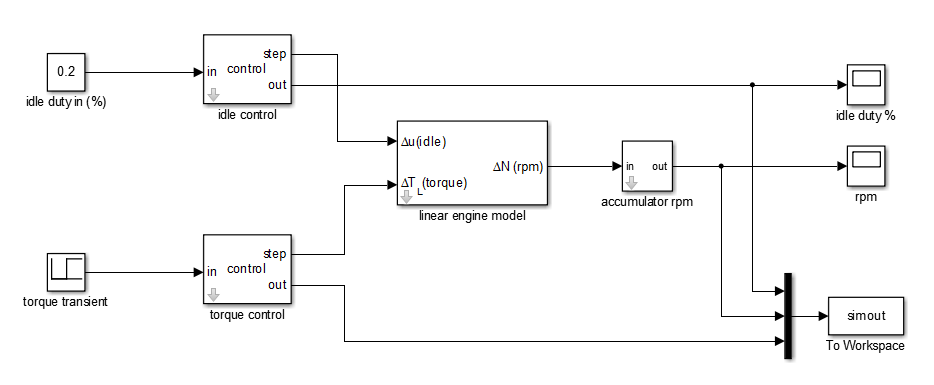
\includegraphics[scale=0.5]{img/schematic-no_control-ed1}
\end{center}
\caption{Linear engine model with an open loop controller.
Inputs go through the simple controller to provide steps to the
engine model.
The output rpm, since it is in steps ($\Delta N$), is accumulated.}
\label{fig:openloop}
\end{figure}

\begin{figure}
\begin{center}
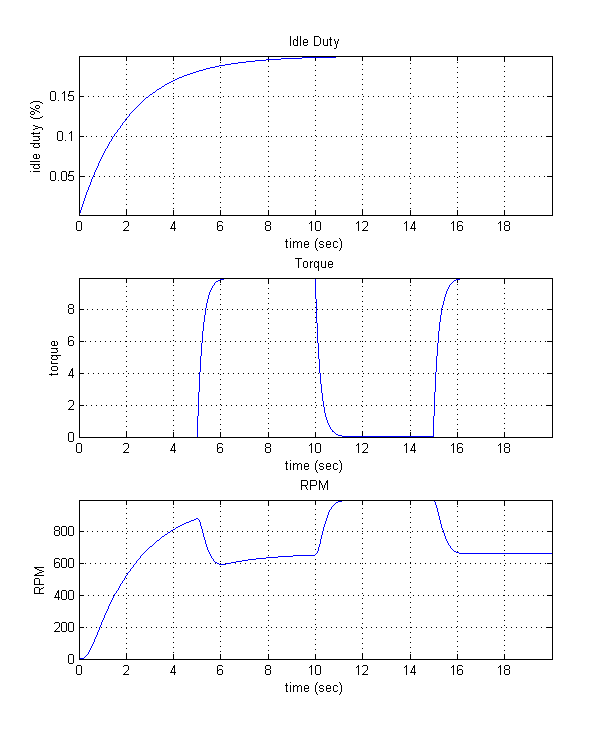
\includegraphics[scale=0.8]{img/linear_engine_model_no_control_plot}
\end{center}
\caption{Output of linear engine controller with a transient torque
input and a fixed input duty cycle.  Matlab source given in
Appendix \ref{app:olplot}}
\label{fig:olplot}
\end{figure}

% References
\clearpage
\printbibliography[heading=bibintoc]

\clearpage
\appendix

% {{{ Steady State to Delta $Z$ Transform Derivation
\clearpage
\section{Steady State to Delta $Z$ Transform Derivation}
\label{app:cdelta}

To accumulate a steady state input to produce a delta output
a system can be constructed as shown in Figure \ref{fig:cd1}.
Its operation can be confirmed by trying some values.
If all values are zero and then a $1$ is input on $u$ the
output will become $1$.
On the next time step $1$ will be output on $v$.
Since $q$ is zero $r$ will be $1$.
If the input ($u$) remains $1$ this will be subtracted from $r$
to produce zero on the output ($y$).

% {{{ fig:cd1
\begin{figure}[hpb!]
\begin{center}

\begin{tikzpicture}[>=triangle 60,
	node distance=14mm, auto]

	\node[sumnp]  	(sum1)	[] 					{};
	\node[sumxpxp] 	(sum2)	[below=of sum1] 	{};
	\node[gain] 	(gain1)	[right=of sum2]		{$z^{-1}$};
	\node[gain] 	(gain2)	[left=of sum2]		{$z^{-1}$};

	\draw [->] (sum2.north) -- 					(sum1.south);
	\draw [->] (gain1.west) -- node[below]{$v$} 	(sum2.east);
	\draw [->] (gain2.east) -- node[below]{$q$} 	(sum2.west);

	 \draw [->]
	 		($ (sum1.south) - (0,7mm) $)
			-- ++(-35mm,0) node[below left,yshift=-3mm]{$r$} 
			|- (gain2.west);
	\draw [->]
			(-45mm,0) node[above] {$u$} to (sum1);
	\draw [->]
			(sum1) to (45mm,0) node[above] {$y$};
	\draw [->]
			($(sum1.east) + (33mm,0) $)
			|- (gain1);
\end{tikzpicture}

\end{center}

\caption{System to accumulate values to convert a steady state
input to a delta output.}
\label{fig:cd1}
\end{figure}

% }}}

Figure \ref{fig:cd1_plot} shows the response of this system given
an arbitrary input.
It can be seen that if the input is held constant the output (delta)
returns to zero as expected.

\begin{figure}[htbp!]
\includegraphics[scale=0.7]{../octave/cd1_plot}
\caption{Response of full steady state input to delta output system
to an arbitrary input signal.
The upper plot is the input signal ($u$) and the lower plot is
the output response ($y$).
The Matlab source code is given in Listing \ref{lst:cd1_init}
and \ref{lst:cd1_plot}.
}
\label{fig:cd1_plot}
\end{figure}

\begin{samepage}
However this full system can be simplified to a single transfer function.
Starting from the equations that define the system
\begin{align}
	r &= q + v \label{eq:cd1a} \\
	v &= y \cdot z^{-1} \label{eq:cd1b} \\
	q &= r \cdot z^{-1} \label{eq:cd1c} \\
	y &= u - r \label{eq:cd1d}
\end{align}
these can be algebraically manipulated to find the effective transfer
function of the entire system ($y/u$).
\end{samepage}

\begin{align*}
	r &= r z^{-1} + y z^{-1} && (\ref{eq:cd1a}, \ref{eq:cd1b}, \ref{eq:cd1c})\\
	r(1 - z^{-1}) &= y z^{-1} \\
	r &= u - y && (\ref{eq:cd1d} \\
	(u - y)(1 - z^{-1}) &= y z^{-1} \\
	u - y - u z^{-1} + y z^{-1} &= y z^{-1} \\
	u - y - u z^{-1} &= 0 \\
	y &= u (1 - z^{-1})
\end{align*}
\begin{align}
	\Aboxed{ \frac{y}{u} &= 1 - z^{-1} }
\end{align}

\begin{figure}[!htbp]
\begin{center}

\begin{tikzpicture}[>=triangle 60]
\node[gain] (gain1) [] {$1 - z^{-1}$};
\draw [->] (-30mm,0) node[above,yshift=1mm]{$u$} -- (gain1.west);
\draw [->] (gain1.east) -- (30mm,0) node[above,yshift=1mm]{$y$};
\end{tikzpicture}

\end{center}
\caption{Simplified system to convert a steady state input in to
a delta output.}
\label{fig:cd1s}
\end{figure}

It can be seen in Figure \ref{fig:cd2_plot} that the simplified system
behaves identically to the previous system (Figure \ref{fig:cd1_plot}).

\begin{figure}[htbp!]
\includegraphics[scale=0.7]{../octave/cd2_plot}
\caption{Response of simplified steady state input to delta output system
to an arbitrary input signal.
The upper plot is the input signal ($u$) and the lower plot is
the output response ($y$).
Response is identical to the full system in Figure \ref{fig:cd1_plot}
as expected.
The Matlab source code is given in Listing \ref{lst:cd2_init}
and \ref{lst:cd2_plot}.
}
\label{fig:cd2_plot}
\end{figure}

\clearpage
\subsection{Matlab Source}
\label{app:cdsrc}

The following code has been tested using Octave\autocite{octave},
an open source Matlab clone.

\lstinputlisting[caption={Matlab code to initialize the full
steady state to delta system.},
	label=lst:cd1_init
	]{../octave/cd1_init.m}

\lstinputlisting[caption={Matlab code to plot the full steady state
to delta system.},
	label=lst:cd1_plot
	]{../octave/cd1_plot.m}

\clearpage
\lstinputlisting[caption={Matlab code to initialize the simplified
steady state to delta system.},
	label=lst:cd2_init
	]{../octave/cd2_init.m}

\lstinputlisting[caption={Matlab code to plot the simplified steady state
to delta system.},
	label=lst:cd2_plot
	]{../octave/cd2_plot.m}

% }}}

\clearpage
\section{Linear Engine Model Plot Matlab Script}
\label{app:olplot}
\lstinputlisting[language=Matlab]{../matlab/linear_engine_model_plot.m}

\section{Linear Engine Model Initialization Matlab Script}
\lstinputlisting[language=Matlab]{../matlab/linear_engine_model_init.m}

\end{document}
